\title{20. Analytická geometrie lineárních útvarů, vektorová algebra}
\author{Michaela Dudašková (Jakub Sláma)}
\date{1.5.2025}

\maketitle

\section{Analytická geometrie lineárních útvarů, vektorová algebra}
- Používáme kartézskou soustavu souřadnic \\
- Bod X má souřadnice $[a,b]$, souřadnice a leží na ose $x$ a souřadnice $b$ leží na ose $y$ je to uspořádaná dvojice hodnot.\\
\begin{figure}[H]
        \centering
        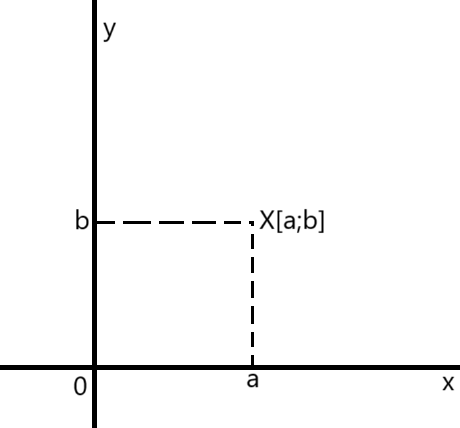
\includegraphics[width=0.4\linewidth]{img/20_kartezka_souradnice.png}
        \caption{Graf kartézské soustavy souřadnic} 
        \label{fig:enter-label}
    \end{figure}

\subsection{Body a vektory}
Pro body $A[x_a;y_a];B[x_b;y_b]$:\\ \\
\subsubsection{Střed úsečky:} 
$$
    S[\frac{x_a+x_b}{2};\frac{y_a+y_b}{2}]
$$ 
\subsubsection{Velikost úsečky:} 
$$
    |AB|=\sqrt{(x_b-x_a)^2+(y_b-y_a)^2}
$$
\subsubsection{Orientovaná úsečka:}
\begin{itemize}
    \item Kromě délky určuje i směr
    \item Určuje počátek a konec
    \item Opačně orientované úsečky mají opačné hodnoty
\end{itemize}
$$
    \overrightarrow{AB}=B-A=(x_b-x_a;y_b-y_a)
$$
$$
    \overrightarrow{BA}=A-B=(x_a-x_b;y_a-y_b)
$$
\subsubsection{Vektor}
\begin{itemize}
    \item Všechny orientované úsečky se stejným směrem a velikostí
    \item Označují se malým písmenem a šipkou
    \item Zobrazují posunutí (o kolik se bod posunul po ose $x$ a $y$)
    \item Kolmé vektory mají hodnoty prohozené a u jedné odlišné znaménko
\end{itemize}
$$
    \overrightarrow{u}=(a;b)
$$
$$
    \overrightarrow{u} \perp \overrightarrow{v}
$$
$$
    \overrightarrow{v}=(b;-a)
$$
\subsubsection{Operace s vektory}
\begin{itemize}
    \item Můžeme násobit vektor libovolným číslem, musíme ale násobit obě souřadnice
    \item Můžeme sčítat a odčítat vektory

$$
    \overrightarrow{u}+\overrightarrow{v}=(x_u+x_v;y_u+y_v)
$$
$$
    \overrightarrow{u}-\overrightarrow{v}=(x_u-x_v;y_u-y_v)
$$
    \item Můžeme vektory násobit – skalární součin
$$
    \overrightarrow{u} \cdot \overrightarrow{v}=(x_u\cdot x_v;y_u\cdot y_v)
$$
\end{itemize}
\subsubsection{Odchylka vektorů (odchylka dvou přímek)}
\begin{itemize}
    \item Odchylka dvou přímek je od $0^\circ$do $90^\circ$- u vektorů neplatí
    \item Odchylka u vektorů je od $0^\circ$ do $180^\circ$ \\
$$
    cos\alpha=\frac{\overrightarrow{u} \cdot \overrightarrow{v}}{|\overrightarrow{u}| \cdot |\overrightarrow{v}|}
$$
    \item Úhel $0^\circ$ svírají dva rovnoběžné a stejně orientované vektory
    \item Úhel $180^\circ$ svírají rovnoběžné a opačně orientované vektory
    \item Rovnoběžné vektory poznáme tak, že jeden je násobek toho druhého
    \item Úhel $90^\circ$ svírají kolmé vektory — skalární součin musí být roven nule
    \item Tzv. Nulový vektor $\overrightarrow{0}=(0;0)$
\end{itemize}

\subsection{Přímky}

\subsubsection{Parametrická rovnice přímky}

\begin{itemize}
    \item Směrový vektor $\overrightarrow{u}$ určuje směr, je rovnoběžný s přímkou
    \item Parametr, který náleží do množiny reálných čísel: $ t \in \mathbb{R} $
    \item Bod $ A $, který leží na přímce
\end{itemize}
$$
    x\in p:x=x_a+t \cdot \overrightarrow{u_x}
$$
$$
    y\in p:y=y_a+t \cdot \overrightarrow{u_y}; t \in \mathbb{R}
$$

\subsubsection{Obecná rovnice přímky}

\begin{itemize}
    \item Alespoň jedno z čísel $a$, $b$, $c$ musí být nenulové, aby rovnice určovala přímku.
    \item Normálový vektor – kolmý na přímku, má souřadnice $(a, b)$.
    \item Bod ležící na přímce má souřadnice $[x, y]$, které splňují rovnici.
$$
    ax+by+c=0
$$
    \item Čísla $a$, $b$, $c$ by měla být nesoudělná (tj. jejich největší společný dělitel je 1).
\end{itemize}

\subsubsection{Směrnicový tvar přímky}
\begin{itemize}
    \item Směrnice = tangens úhlu mezi přímkou a kladnou poloosou $x$.
    \item Přímka rovnoběžná s osou $y$ nemá směrnicový tvar!
    $y=kx+q$
    $k=tg\alpha$
\begin{figure}[H]
        \centering
        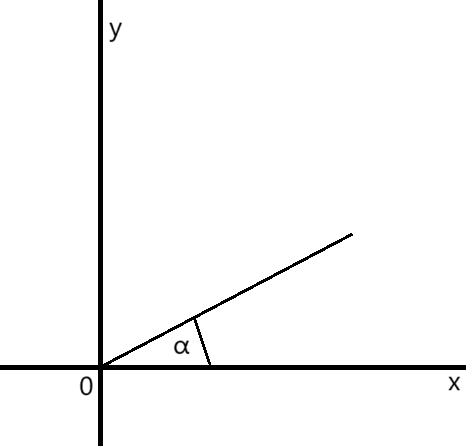
\includegraphics[width=0.2\linewidth]{img/20_kartezka_alfa.png}
        \caption{Graf směrnicové přímky} 
        \label{fig:enter-label}
    \end{figure}
\end{itemize}

\subsubsection{Polopřímky}

\begin{itemize}
    \item Stačí u parametrické rovnice přímky zadat interval, ze kterého budeme parametr vybírat.
$p:$
$$
    x=a_x+t\cdot u_x
$$
$$
    x=a_y+t\cdot u_y; t \in (z;r)
$$
Kdy $z$ označuje začátek intervalu a $r$ konec. Intervaly mohou být otevřené i zavřené.
\end{itemize}

\subsubsection*{Bod a přímka}

\begin{itemize}
    \item Pro zjištění, zda bod leží na přímce, dosadíme souřadnice bodu za $x$ a $y$ do rovnice přímky.
    \item Vzdálenost bodu od přímky lze spočítat pomocí speciálního vzorce.
\end{itemize}
$$
    p: ax+by+c=0
$$
$$
    M=[m;n]
$$
$$
    V_{M,p}=\frac{|a\cdot m+b \cdot n + c|}{\sqrt{a^2+b^2}}
$$

\subsubsection{Vzájemná poloha dvou přímek v rovině}
\begin{itemize}
    \item Vzájemnou polohu zjistíme pomocí soustavy rovnic.
    \item Možnosti:
    \begin{itemize}
        \item \textbf{Totožné} – jedna rovnice je násobkem druhé, výsledkem je nekonečně mnoho společných bodů.
        \item \textbf{Rovnoběžné} – soustava nemá řešení, přímky se nikdy neprotínají.
        \item \textbf{Různoběžné} – soustava má právě jedno řešení, přímky se protínají v jednom bodě.
    \end{itemize}
\end{itemize}
